%!TEX root = ../Master Thesis.tex

\chapter{Introduction} % (fold)
\label{cha:introduction}

Introduction of chapter, overview, \ldots

\section{Motivation}
\label{sec:motivation}

\begin{quotation}
  \textit{\enquote{When it comes to fraud, 2015 is likely among the riskiest season retailers have ever seen, […]
  it is critical that they prepare for a significant uptick in fraud, particularly within e-commerce channels.}}
\end{quotation}
This statement from Mike Braatz, senior vice president of Payment Risk Management, ACI Worldwide in \citep{Reuters2015}
shows the dramatic shift in credit card fraud from the offline to the online world, that retailers are starting to face
nowadays. \\

In general credit card fraud can occur if a consumer has lost her credit card or if the credit card has been stolen
by a criminal. This usually results in an \textbf{identity theft} by the criminal, who is using the original credit card
to make financial transactions by pretending to be the owner of the card. Additionally, a consumer might hand over her
credit card information to an untrustworthy individual, who might use this information for her own benefit.
In the real world scenario there is usually a face-to-face interaction between both parties.
The consumer, wanting to do business with a merchant or interacting with an employee of a larger business, has to hand over
her credit card information explicitly and can deny doing so if she faces a suspicious situation.
The criminal on the other hand must get access to the physical credit card first, before she is able to make an
illegal copy of it --- a process called \textbf{skimming}. The devices used to read out and duplicate the credit card
information are therefore called skimmers. These can be special terminals, that the criminal uses to make copies of
credit cards she gets her hands on, or they can be installed in or attached to terminals the consumer interacts with on her own
\citep{ConsumerAction2009}. All of these so-called \textit{card-present transaction} scenarios have seen a lot of improvements in security
over the last years. Especially the transition from magnetic swipe readers to EMV chip-based credit cards makes it more difficult
for criminals to counterfeit them \citep{Lewis2015}. \\

As of this criminals are turning away from these card-present transaction scenarios in the offline world. Instead they are focusing on transactions
in the online and mobile world, in which it is easy to pretend to own a certain credit card. Most online transactions (either e-commerce or m-commerce)
rely \textbf{\textit{only}} on credit card information like card number, card holder and security code for the card validation process – as of this these interactions
are usually called \textit{card-not-present transactions}. This credit card information can be obtained by a criminal in a number of ways.
First she might send out \textbf{phishing emails} to consumers. These emails mimic the look-and-feel of emails from a merchant or bank, that the consumers are normally
interacting with, but instead navigating the consumers to a malicious web site with the intend to capture credit card or other personal information \citep{ConsumerAction2009}.
Additionally, criminals can \textbf{break into the web sites} of large Internet businesses with the goal of getting access to the underlying database of customer information,
that in most cases also hold credit card data \citep{Holmes2015}. Additionally, some of the online retailers are not encrypting the transaction information before transmitting
them over the Internet; a hacker can easily start a \textbf{man-in-the-middle attack} to trace these data packages and get access to credit card and/or personal information
in this way \citep{Captain2015}. \\

Based on this it should come not as a surprise that the growth rate of online fraud has been 163\% in 2015 alone \citep{PYMNTS2016}.
This results in huge losses for the global economy every year and it is expected that retailers are losing \$3.08 for every dollar in fraud incurred in 2014
(incl.\ the costs for handling fraudulent transactions) \citep{Rampton2015}. These fraudulent transactions also impact the revenue of the online retailers.
Here we have seen a growth of 94\% in revenue lost in 2015. Overall it is estimated that credit card fault results in \$16 billion losses globally in 2014 \citep{PYMNTS2016}
\citep{BusinessWire2015}. \\

While it is possible to prevent fraudulent transactions in the card-present real-world scenario (mainly due to introducing better technology and establishing organizational
countermeasures in the recent past), it is more difficult to do so in the card-not-present online- and mobile commerce scenarios, which are lacking face-to-face interactions
and enable massive scalability of misusing credit card information in even shorter time frames \citep{Lewis2015}. Large online retailers have tried to establish countermeasures
and transaction data analysis technologies to lower the rate of fraudulent transactions to a manageable amount. But this is still an expensive and inefficient solution to integrate
into the retailers’ business processes, and is largely driven by machine-learning techniques and manual review processes \citep{Brachmann2015}. Additionally, it can be assumed,
that the online retailers are getting into a Red Queen race with the criminals here: with every new technology or method introduced they might just be able to safe the status quo.
This is largely due to the facts, that there will be no 100\% security for such a complex and interconnected system like an e-commerce or m-commerce shop, the criminals will also
increase their efforts and technology skills to adapt to new security features and most importantly retailers will always have to make a trade-off between the \textit{performance}
of the transaction processing, the \textit{usability} of the web shop and the overall \textit{security} of it.

% section motivation (end)

\section{Problem Definition}
\label{sec:problem_definition}

This Master thesis will \textbf{\underline{not}} look into novel techniques and methods to \textit{prevent} credit card fraud in the e-commerce world. This aspect has been seeing a lot of research
in the last years.\footnote{please also note the various US patent applications of Google on that matter from 2015, e.g.:\ “Credit card fraud prevention system and method”, “Financial card fraud alert”,
“Payment card fraud prevention system and method” \citep{GooglePatents2015}} Instead this Master thesis will look into a \textbf{concept to optimize the collaboration} between the affected stakeholders in case of an existing credit card fraud in an e-commerce system. \\

Stakeholders might include \textbf{vendors} and other businesses, that the retailer has a long-term business relationship with, \textbf{law enforcement agencies}, \textbf{acquirers} like PayPal or Visa,
and even \textbf{competitors}, that are also affected by the Internet fraud. In such a case the merchant usually tries to solve the issue on his own and getting in contact with relative parties by phone or e-mail
if necessary. But these communication styles do not fit to the complexity of the task involved, and based on the media-richness model (see Figure~\ref{fig:images_media_richness_model}) will result in inefficient and ineffective problem solutions.

\begin{figure}[H]
	\centering
		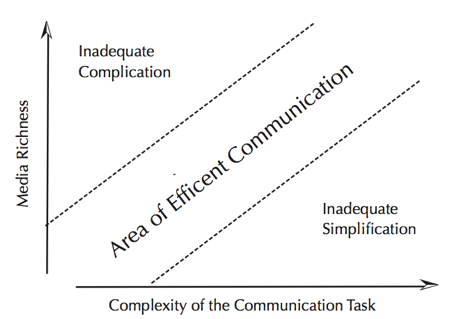
\includegraphics[height=3in]{images/media-richness-model.png}
	\caption{The Media Richness Model \citep{Rice1992}}
\label{fig:images_media_richness_model}
\end{figure}

Due to the task complexity a \textbf{physical face-to-face meeting} with representatives of all involved stakeholders might be a good fit, but arranging such a meeting (same time, same place) with multiple parties,
that are globally dispersed, is either economically not feasible or takes a lot of time. But the more time passes for investigating the crime the more difficult it will become to find the criminals and take legal actions against them,
which can also reduce the risk of losing the stolen money completely. \\

As of these conditions a \textbf{computer-supported collaborative work} (CSCW) system might be an alternative to \textit{cooperate} on an incident of e-commerce fraud (same time, different place).
CSCW systems can be categorized by their support for the mode of group interaction as done in the 3C model:

\begin{itemize}
    \item\textbf{communication:} two-way exchange of information between different parties
    \item\textbf{coordination:} management of shared resources like meeting rooms
    \item\textbf{collaboration:} members of a group work together in a shared environment to reach a goal
\end{itemize}

Based on the level of support for one of these functionalities the various systems can be classified and described (see Figure~\ref{fig:images_3C_model}) \citep{Koch2008}:

\begin{figure}[H]
	\centering
		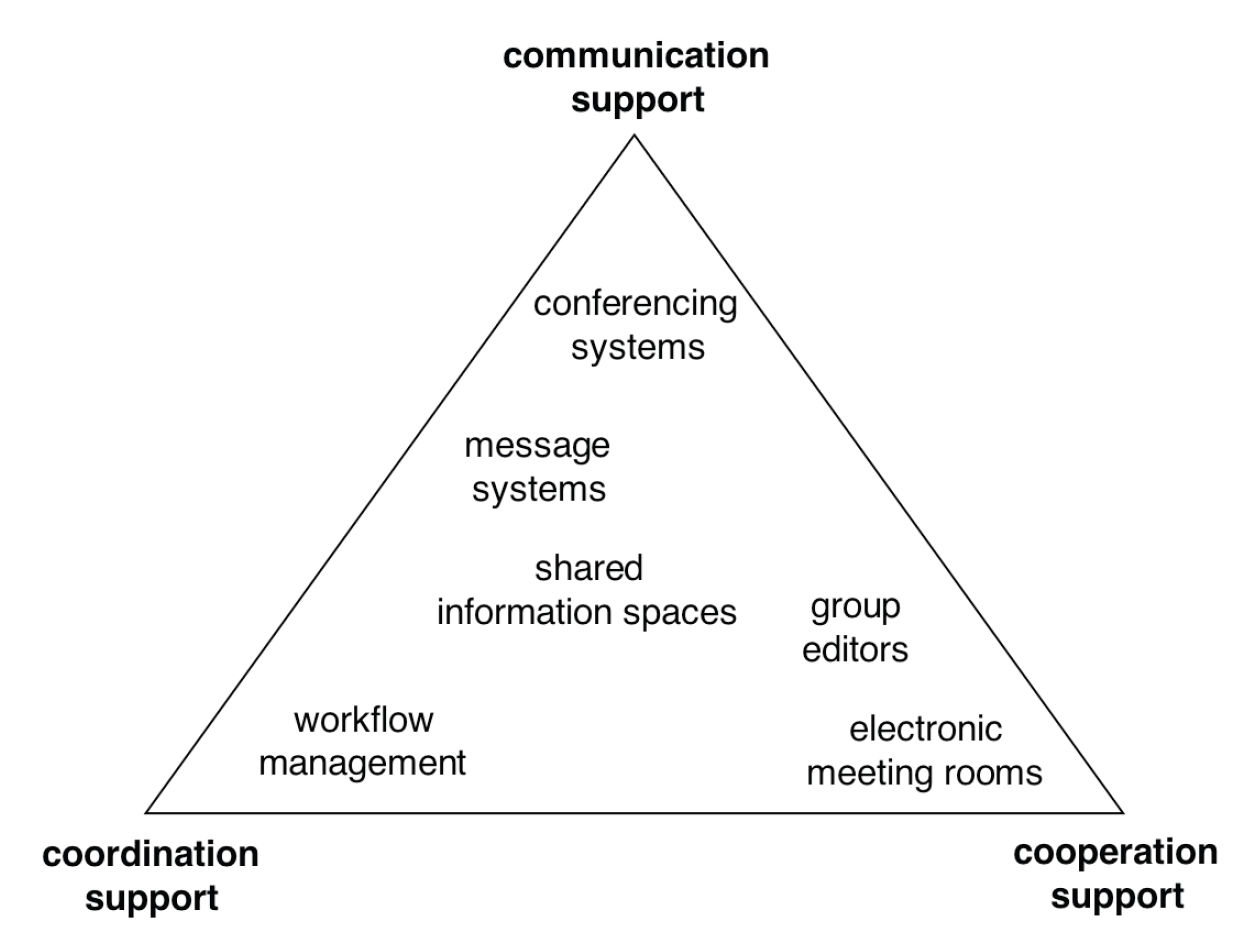
\includegraphics[height=3in]{images/3C-model.png}
	\caption{The 3C Model \citep{Koch2008}}
\label{fig:images_3C_model}
\end{figure}

A good candidate \textit{could} be a \textbf{shared information space}; aka team rooms, cloud storage services or document management systems, that allow to access information at any place,
any time and to share information with co-workers --- usually with a build in versioning support for artefacts and a workflow component. \\

However as some of the required information might be confidential or business-critical to one of the involved parties a \textbf{centralized system} (e.g.\ a service in the cloud) could \textbf{\underline{not}} be used in the scenario described here.
Another key characteristic of the investigation of an e-commerce fraud is, that it involves information sharing from many different organizations. These different aspects have to be combined into a \textbf{shared information space} in a meaningful way
to be able to achieve the common group goal on time. Combining information from different stakeholders will face issues due to \textbf{different wordings and data formats} of the information,
\textbf{competing incentives} of the stakeholders to participate on information sharing as well as possible \textbf{sharing restrictions}, that prevent making the information available to a larger audience (e.g.\ via an Open Data Initiative). \\

\textbf{Decentralized information sharing architectures}, that utilizes \textbf{peer-to-peer communication technologies}, are either restricted to a commonly agreed set of data entities and relations (based on an ontology) between all involved parties
or are lacking richer semantics for sharing and integrating content between the stakeholders. \textbf{Semantic Web technologies} can help lower the barrier to integrate information from various sources into a shared information space,
and the advantages of peer-to-peer communication and Semantic Web technologies for information sharing in distributed, inter-organizational settings have been shown in \citep{Staab2006}. \\

Still these studies concentrate on making information from different parties searchable and accessible in a distributed, shared information space, which data can be accessed and queried at any time from any participating party.
They are not solving the problem of working collaboratively on a common goal in an ad-hoc, loosely-coupled virtual team of disperse organizations by making certain (sometimes sensitive) information available in a shared environment. \\

Therefore, the \textbf{research question} for this Master thesis can be summarized as:
\begin{quotation}
  \textit{In how far can a computer supported collaborative work system based on peer-to-peer communication technologies and shared ontologies improve the efficiency and effectivity of e-commerce fraud investigations within an inter-institutional team?}
\end{quotation}

% section problem definition (end)

\section{Related Works}
\label{sec:related_works}

% section related works (end)

\section{Thesis Outline}
\label{sec:thesis_outline}

% section thesis outline (end)

% chapter introduction (end)
